\documentclass[conference,a4paper]{IEEEtran}
\usepackage[utf8]{inputenc}
\usepackage{booktabs}
\usepackage{enumitem} %resume enumerate
\usepackage{graphicx}
\usepackage{caption}
\usepackage{subcaption}
\usepackage{hyperref}
\usepackage{url}
\usepackage[x11names, svgnames, rgb]{xcolor}
\usepackage{amsmath}
\usepackage{balance}

\def\BibTeX{{\rm B\kern-.05em{\sc i\kern-.025em b}\kern-.08em
    T\kern-.1667em\lower.7ex\hbox{E}\kern-.125emX}}

\begin{document}

\title{DNA Pattern Matching}

\author{\IEEEauthorblockN{Roger Pujol}
\IEEEauthorblockA{\textit{Universitat Politècnica de Catalunya (UPC)}\\
Barcelona, Spain \\
roger.pujol.torramorell@est.fib.upc.edu}}

\date{\today}

\maketitle

\begin{abstract}
In this project I am going to analyze 4 of the most used algorithms used to find patterns in a DNA sequence.

The code of this project is Open Source and can be found in: \url{https://github.com/rogerpt32/dna_pattern}.
\end{abstract}

\section{Summary}
The algorithms that I analyzed are:
\begin{itemize}
    \item Bruteforce
    \item Horspool
    \item Backward Nondeterministic Dawg Matching (BNDM)
    \item Backward Oracle Matching algorithm (BOM)
\end{itemize}
The data we used to test this algorithms is a portion of the Human genome.
\section{implementation}
First I coded a script to simplify the format of the genome, remove all characters different to `A', `C', `G' and `T'. Also it deletes some blocks of the sequence in order to fit it in 2 GB (this is needed because the implementations given couldn't handle all the 3 GB file).
Then I adapted the implementations from the web page \url{http://www-igm.univ-mlv.fr/~lecroq/string/index.html}, in order to make them work properly and print the output with the same format. After that I implemented a small program that generates a random sequence of a specified length. Using all these binaries, I created a bash script that for every length between 1 and 32 generates the pattern and runs every algorithm, while storing their outputs. After that calls another script which merge all the outputs in a single csv file. Finally with another script, we use the data in the csv to generate all the plots.

\section{Results}
Here are the plots that show the results of the experiments. Figure \ref{fig:time_len} shows how in Hosrpool, BNDM and BOM, the execution time decreases with the length of the pattern whereas in the Bruteforce there is no clear relation (the time is almost constant). In figure \ref{fig:alg_len} shows that for very small patterns the best is Bruteforce, then for patterns between 4 and 8 the best is Hosrpool and for bigger patterns the best one is BNDM. Finally in figures \ref{fig:matches_len} \& \ref{fig:matches_len2}, we see how the number of matches in the sequence have an exponential decay, which in our particular case hits 0 for patterns with more than 16 characters.

\section{Conclusions}
In conclusion, according to this results we should use Bruteforce to find patterns of less than 4 characters long, Hosrpool for patterns between 4 and 8 characters and BNDM for anything longer than 8 characters. Also we can see that for a 2GB long DNA sequence, the probabilities of finding a random 16 characters or longer pattern are very low.

\begin{figure}[hbp]
    \centering
    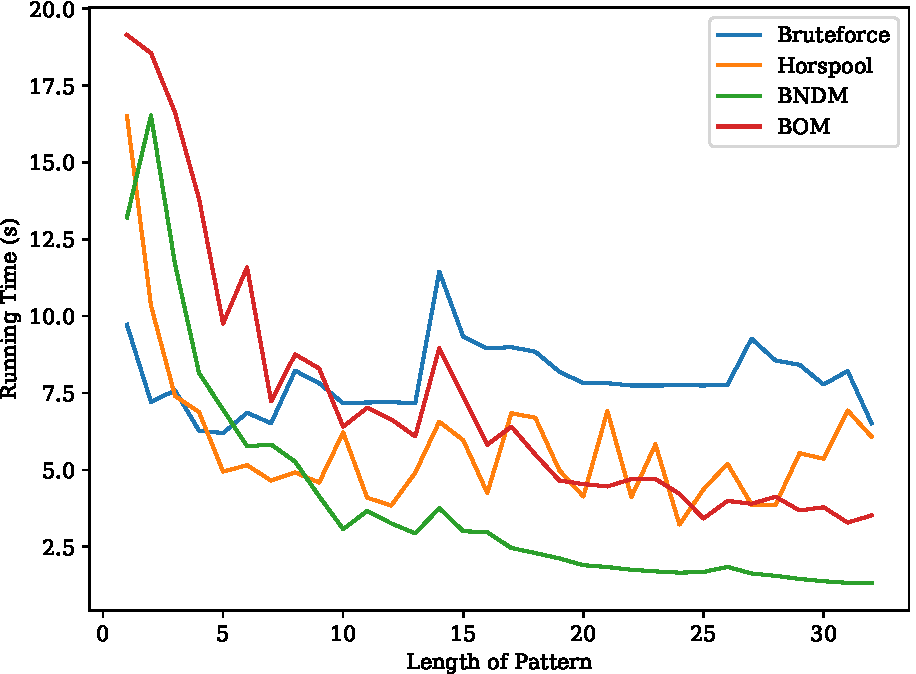
\includegraphics[width=0.95\linewidth]{../plots/time_len.pdf}
    \caption{Plot of the execution times / pattern length, for each algorithm.}
    \label{fig:time_len}
  \end{figure}
  \begin{figure}[hbp]
    \centering
    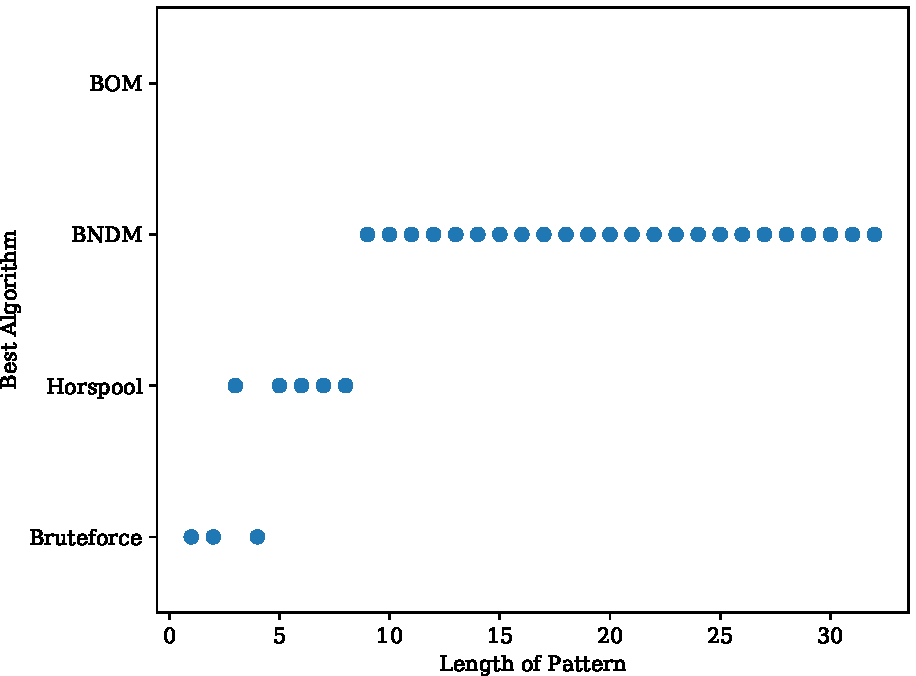
\includegraphics[width=0.95\linewidth]{../plots/alg_len.pdf}
    \caption{Plot of the best algorithm for each pattern length.}
    \label{fig:alg_len}
  \end{figure}
  \begin{figure}[htbp]
    \centering
    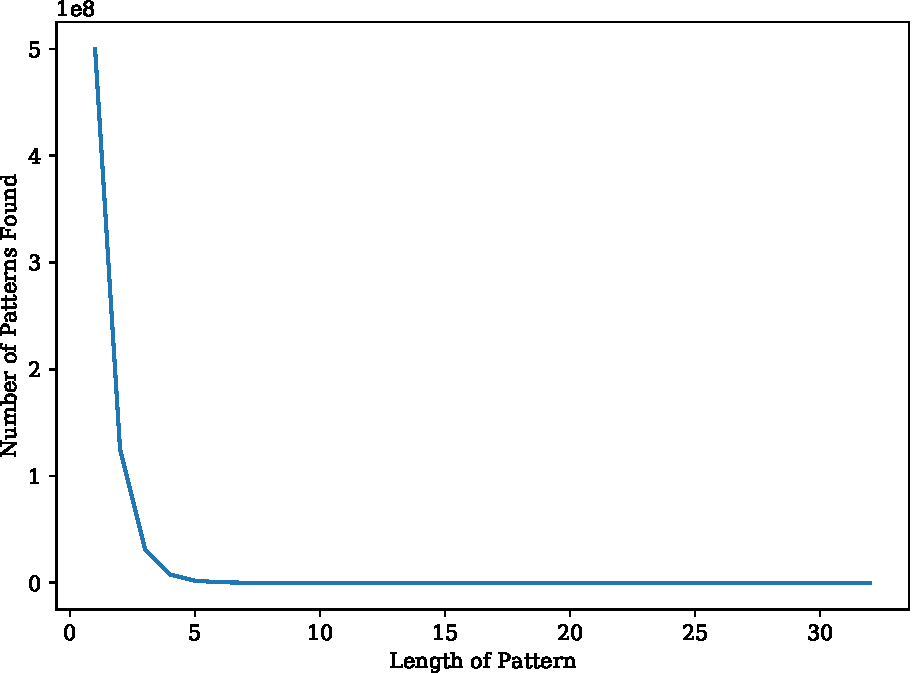
\includegraphics[width=0.95\linewidth]{../plots/matches_len.pdf}
    \caption{Plot of number of patterns found / pattern length.}
    \label{fig:matches_len}
  \end{figure}
  \newpage
  \balance
  \begin{figure}[htbp]
    \centering
    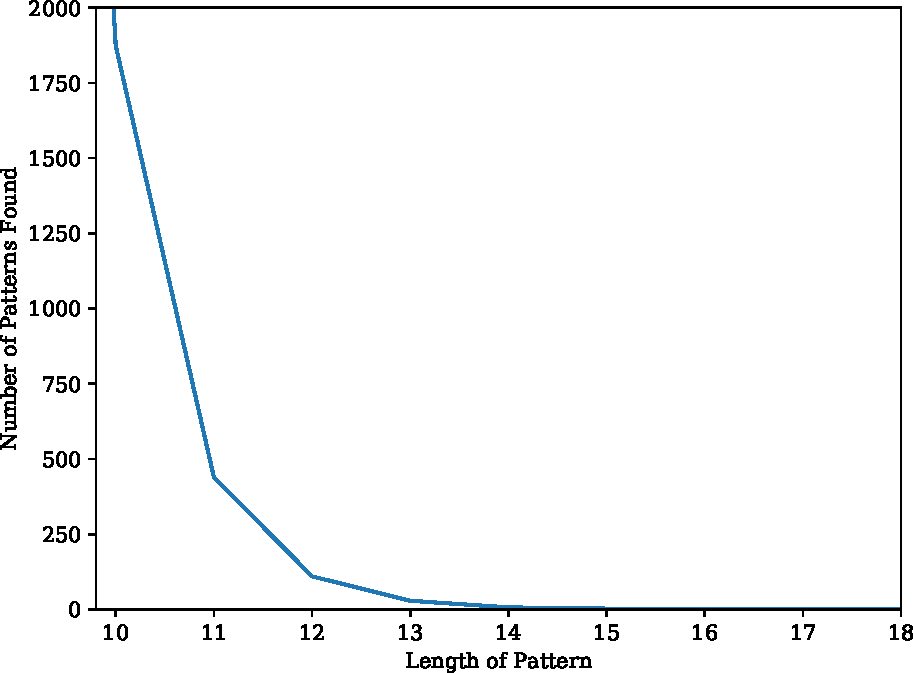
\includegraphics[width=0.95\linewidth]{../plots/matches_len2.pdf}
    \caption{Plot of number of patterns found / pattern length, only patterns of size between 10 and 18.}
    \label{fig:matches_len2}
  \end{figure}


% \bibliographystyle{unsrt}
% \bibliography{cites}


\end{document}